\clearpage
\onecolumn
\section{Interpreting Attention Measurements}
\label{sec:supp-attention-views}
How should attention measurements of a perturbation be read? Which layer changes more, and whether the change grows during generation, depend on the image region, the computation site and the reference scale. This section and Sec.~\ref{sec:supp-attention-analysis} are an additional study; the main paper mentions it once, in Related Work, and does not rely on it. Figures~\ref{fig:supp-attention-spatial-main-view} and~\ref{fig:supp-attention-main-view} give a spatial example and the complete generation profiles (trends: Fig.~\ref{fig:attention-trends}; regional comparisons: Table~\ref{tab:legacy-attention}; definitions and checks: Secs.~\ref{sec:plus-sites} and~\ref{sec:supp-protocol-validation}).

Image-region interventions estimate visual-action attribution~\cite{zhang2026embodied}, and attention-output patching tests language perturbations~\cite{wulff2026language}. We therefore examine both attention probabilities and the output vectors that combine them with transformed values. For a state $H$, the relative difference is $\|H^p-H^c\|_F/\|H^c\|_F$, pooled over the selected positions and channels.

\paragraph{Regional attention needs its total mass as context.}
In a separate 36-task study, rotating only the main camera changes deep wrist features although wrist pixels, physical state and instruction are fixed, and attention redistributes within the unchanged wrist image. The redistribution appears larger at L18 than at L9, but weighting it by the wrist's share of all attention reverses the ranking (Sec.~\ref{supp:legacy-attention} and Table~\ref{tab:legacy-attention}).

\paragraph{The measurement site changes the generation trend.}
On the 404 matched $\pi_{0.5}$ pairs at L18, recomputed attention probabilities of the clean and perturbed runs become closer from generation step 0 to 9, while the projected outputs, which combine probabilities with transformed values~\cite{kobayashi2020} and are measured before gating, move apart. Block-end states recorded during the policy's own generation show smaller absolute but larger relative differences; they include the residual and feed-forward updates, a different stage (Sec.~\ref{sec:plus-sites}).

The recomputation runs the frozen blocks on each run's saved generation state. A check on one input at three steps matches the recorded hidden states, with 0.37--0.46\% relative velocity error. Probabilities and projected outputs were not recorded during generation, so they could not be compared directly (Secs.~\ref{supp:recording-overview} and~\ref{sec:supp-protocol-validation}).

\paragraph{Probabilities and outputs show no clear difference in their link to commands.}
The difference between the command associations of $P$ and $W$ has intervals that include or touch zero in all four families (Sec.~\ref{sec:supp-bounded-internal}, Fig.~\ref{fig:supp-attention-estimates}b and Table~\ref{tab:supp-internal-links}). The generation finding concerns their different profiles: read together, probabilities, outputs and block-end states show changes a single attention map does not.

\clearpage
\begin{center}

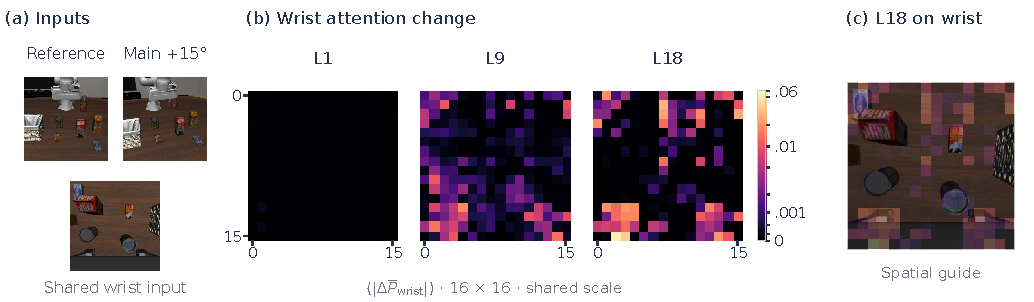
\includegraphics[width=0.90\textwidth]{current_figures/figure4.pdf}
\captionof{figure}{\textbf{Attention is redistributed over an unchanged wrist image.}
One $\pi_{0.5}$ example, recomputed at generation step 5 with the same plan state, generation time and policy noise in both runs.
(a) A $15^\circ$ main-camera change holds wrist pixels, physical state, and instruction fixed.
(b) Wrist probabilities are normalized to sum to one: $\widetilde P_{\mathrm{wrist}}=P_{\mathrm{wrist}}/m$. Heatmaps show mean absolute changes over eight heads and ten plan positions, with a shared asinh scale. Brightness indicates change magnitude, regardless of sign.
(c) The L18 overlay provides spatial context; the unmixed heatmaps carry quantitative values.
Signed maps: Figure~\ref{fig:attention-spatial-full}.}
\label{fig:supp-attention-spatial-main-view}
\end{center}

\begin{center}

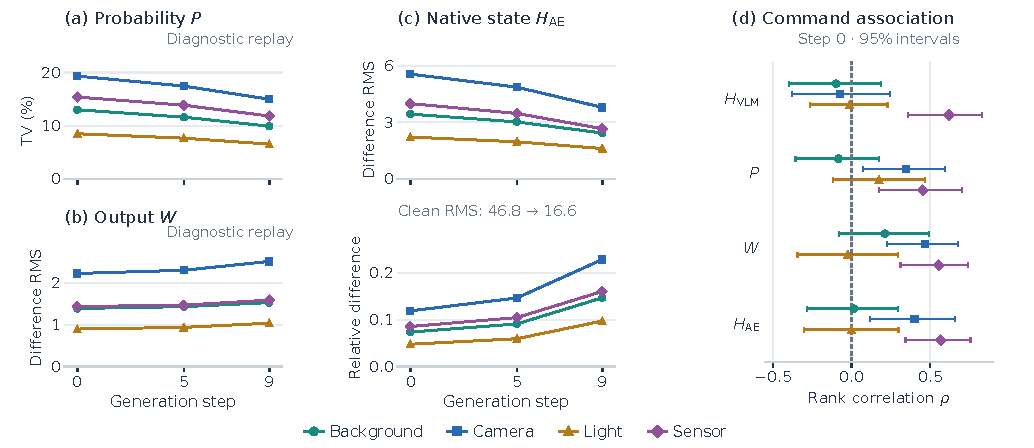
\includegraphics[width=0.90\textwidth]{revised_figures/figure5.pdf}
\captionof{figure}{\textbf{Attention weights, projected outputs and block-end states follow different trends.}
L18 measurements on $404$ $\pi_{0.5}$ LIBERO-Plus pairs from $28$ tasks.
(a,b) Recomputed at each run's saved generation state: full-key probability TV decreases while raw projected-output RMS differences grow.
(c) Block-end states $H_{\mathrm{AE}}$ recorded during the policy's own generation: differences shrink in raw RMS but grow relative to the clean state.
Generation profiles use steps $0/5/9$ of the first query; relative responses are formed per case before task-equal averaging.
(d) Post hoc, step-0 task-centered rank correlations with the RMS change of the first five commands (translation), with pointwise $95\%$ task intervals for each correlation. Here $P$ uses full-key TV and the other measures use clean-relative norms; $H_{\mathrm{VLM}}$ uses main-camera tokens.}
\label{fig:supp-attention-main-view}
\end{center}
